\section{Introduction}
\label{sec:introduction}
The following section is based on my old report about the photoelectric effect, which in turn is
based on the experimental manual for the lab given out by TU Dortmund University. Unfortunately,
both of these are only available in German.

\subsection{Physical theories of light}
\label{sec:intr:theory}
To explain different phenomena with light, physicists developed two different theories in the
history. Processes like diffraction and interference have been explained by seeing light as waves,
while Compton scattering or pair production assume discrete photons. 

The two pictures are incompatible with each other, and they also have different mathematical
descriptions. The photon`s movement is described by Newtonian or relativistic equations for
point like particles, whereas the wave nature is derived from Maxwell`s equations. The theory
combining the two cases is referred to as quantum electrodynamics, and the two cases (point- and 
wave-like) are contained as limiting cases.

Most important for this experiment is, that for light-matter interaction the picture of discrete
photons is performing well enough. For that reason, we can limit ourselves to this theory to get a
meaningfull understanding of the photoelectric effect.

\subsection{The photoelectric effect and it`s explanation using the photon model}
\label{sec:intr:photoeffect}
The photoelectric effect is commonly referred to electrons being emitted from metal when its being
irradiated with light. The first qualitative description has been done by Einstein in 1905
\cite{https://doi.org/10.1002/andp.19053220607}, which also interpreted light as discrete energy
packets.

\begin{figure}
    \centering
    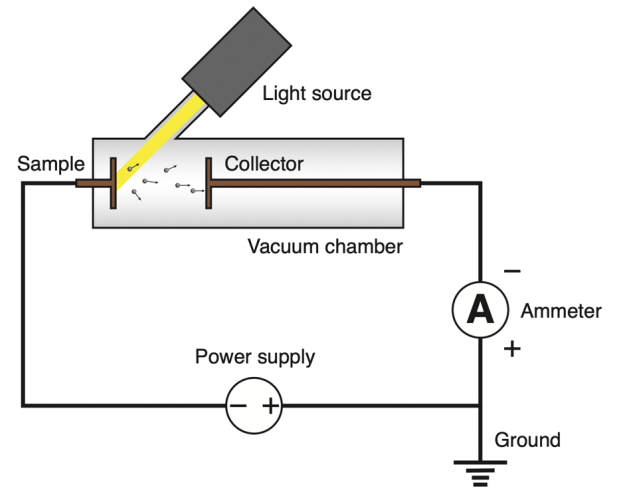
\includegraphics[width=0.4\textwidth]{media/ExperimentalSetup.png}
    \caption{Experimental Setup}
    \label{fig:ExpSetup}
\end{figure}

